% =========================================================================
% When Does Feedback Help? Planning and Model Mismatch in Hessian-Free
% Newton Control
%
% **표현 계층이다.** 내용의 source of truth 는 `paper/draft.md` 다.
% 주장 강도는 `paper/claim_ledger.md` 가 통제하고, 인용 내용 검증은
% `paper/CITATIONS.md` 에 있다.
%
% 규칙
%   1. 표의 숫자를 이 파일이나 sections/ 에 쓰지 않는다.
%      `scripts/make_tables.py` 가 `tables/*.tex` 를 생성한다
%   2. 그림은 `scripts/make_figures.py` 가 생성한다
%   3. 새 주장을 여기서 만들지 않는다. draft.md 에 없는 문장을 넣지 않는다
%
% 빌드
%   pdflatex main && bibtex main && pdflatex main && pdflatex main
% =========================================================================
\documentclass[11pt]{article}

\usepackage[utf8]{inputenc}
\usepackage[T1]{fontenc}
\usepackage[english]{babel}
\usepackage{lmodern}
\usepackage{microtype}

\usepackage[margin=1in]{geometry}
\usepackage{amsmath,amssymb}
\usepackage{booktabs}
\usepackage{tabularx}
\usepackage{graphicx}
\usepackage{subcaption}
% float 이 자기 절 제목을 추월하지 못하게 막는다. `[t]` 만 쓰면 표가 페이지 최상단으로
% 올라가 제목 위에 놓인다 (§9 의 Table 7 이 그랬다). 절 경계에서 float 를 flush 한다.
\usepackage[section]{placeins}
% placeins 의 `section` 옵션은 \section 에만 barrier 를 넣는다. 표만 있는 절
% (§7.4 Search cost, §10.2 Results, §11.3 Results) 은 subsection 단위라 barrier 가
% 없으면 표가 제목을 앞지른다. \subsection 에도 같은 barrier 를 넣는다.
\let\rlnOldSubsection\subsection
\renewcommand{\subsection}{\FloatBarrier\rlnOldSubsection}
% barrier 를 넣으면 표만 있는 절의 제목이 페이지 맨 아래에 고아로 남는다. 제목 뒤에
% 최소 공간을 요구해서 제목과 내용이 갈라지지 않게 한다.
\usepackage{needspace}

% 마지막 수단으로 줄 늘림을 조금 허용한다. §12.1 의 enumerate 항목 한 줄이 들여쓰기
% 때문에 4.96pt 넘쳤다. 문장을 고치는 대신 조판으로 닫는다. 값이 커지면 줄이 헐거워
% 지므로 1em 로 제한하고, Underfull 이 생기지 않는지 빌드 로그로 확인한다.
\setlength{\emergencystretch}{1em}
\usepackage{xcolor}
\usepackage[numbers,sort&compress]{natbib}
\usepackage[hidelinks]{hyperref}

\graphicspath{{figures/}}

% 컨트롤러 이름을 본문에서 일관되게 쓴다.
\newcommand{\ctrl}[1]{\texttt{#1}}
\newcommand{\GE}{\text{GE}}
\newcommand{\JE}{J_E}

% 사전 등록 게이트 표기.
\newcommand{\gate}[1]{\textsf{#1}}

% 아직 존재하지 않는 값의 자리. **눈에 보이게** 조판한다. 조용히 비워 두면 존재하지
% 않는 태그나 URL 을 실재하는 artifact 처럼 제시하는 사고가 난다(E12 와 같은 유형).
% scripts/check_latex.py 가 이 표시를 검출하고 --strict 에서 실패한다.
% 공개 전에 남은 자리가 0 이어야 한다.
\newcommand{\PLACEHOLDER}[1]{\textbf{[TO BE FILLED: #1]}}

\title{When Does Feedback Help?\\
Planning and Model Mismatch in Hessian-Free Newton Control}

\author{%
  Jin-Uk Kim \\
  Department of Data Science \\
  Hanyang University \\
  Seoul, Republic of Korea \\
  \texttt{jwkim628@gmail.com}
}
% 이 문서의 지위를 표지에서 명시한다. 조판된 PDF 만 따로 돌아다닐 때 심사를 통과한
% 논문으로 오독되는 것을 막는다. 날짜를 `\today` 로 두지 않는 이유는 빌드할 때마다
% PDF 가 달라져 재현성이 깨지기 때문이다.
\date{Technical report, August 2026\\[4pt]
  \normalsize Unrefereed. This document has not been peer reviewed and is not
  available from any preprint server.}

\begin{document}
\maketitle

% draft.md Abstract 에 대응한다. CLAIM: scope, C07, C03, C04, C12
\begin{abstract}
We study the allocation of damping and conjugate-gradient (CG) effort in
Hessian-free Newton--CG \citep{martens2010hessianfree,nash2000survey} as a
sequential decision problem, and ask whether the resulting benefit comes from
multi-step planning or from execution-time state feedback.

Under a fixed budget of $150$ gradient-equivalent units (GE) we compare, on the
same ladder, a tuned constant setting, a resource-clock open-loop schedule, a
one-step greedy controller, a planner that commits to a single plan formed at
the initial state, and a planner that replans at every step. The configuration
was fixed once on development seeds and measured on disjoint held-out seeds.

On $40$ instances of ill-conditioned symmetric positive definite quadratics
($d = 100$, $\kappa \in \{10^3, 10^4, 10^5, 10^6\}$, ten held-out seeds each),
multi-step lookahead improved over one-step greedy control by
$+0.456$~nat (95\% CI $+0.254$ to $+0.720$, $p < 0.0001$, $35/40$ instances).
On the same $40$ instances, replanning during execution differed from the
committed planner by $+0.010$~nat (95\% CI $-0.033$ to $+0.053$, $p = 0.97$,
$21/40$). The confidence interval was narrow and included zero, and
\emph{we did not observe a practically large feedback benefit}.

As an exploratory extension we compared a micro-neural problem in a
deterministic full-batch regime and in minibatch regimes, changing only the
samples the optimizer observes for the same model and data
($n = 3$ per regime). In the minibatch regimes, holding a stale plan was
costly and replanning reduced that cost, but \emph{the planner did not
consistently outperform inexpensive one-step control}. Policy learning was a
predeclared conditional next stage; on this evidence we did not proceed to it.
\end{abstract}

\section{Introduction}
\label{sec:intro}

Truncated or inexact Newton methods solve the Newton system approximately with an
iterative solver rather than forming the Hessian
\citep{dembo1982inexact,steihaug1983cg,nash1984lanczos,nash2000survey}.
Implementations that access curvature only through Hessian-vector products build
on the exact product of \citet{pearlmutter1994hvp}; applications at deep-network
scale are reported by \citet{martens2010hessianfree,martens2011rnn}. Practical
performance depends strongly on two computational-resource decisions: the
damping level and the per-step CG iteration budget.

Damping belongs to the Levenberg--Marquardt family of regularizers
\citep{levenberg1944,marquardt1963} and is related to a trust-region radius
\citep{steihaug1983cg,conn2000trustregion}. In Hessian-free optimization the
damping update rule is reported to drive performance
\citep{martens2010hessianfree,martens2011rnn}. Truncating the CG budget is the
central design variable of inexact Newton methods
\citep{dembo1982inexact,nash2000survey}.

Attempts to adapt these two quantities during optimization rather than fixing
them connect to the learned-optimizer literature
\citep{andrychowicz2016l2l,metz2019pathologies,metz2020effective,bae2022apo}.
For reinforcement learning \citep{schulman2017ppo} to be the right tool for
learning such a controller, observing the state and changing the action in
response must carry value. The distinction between fixing a plan in advance and
reacting to the state during execution is the classical distinction between
open-loop and closed-loop control \citep{bertsekas2017dp}.

Our question is not whether performance improves, but \emph{where the
improvement comes from}.

\begin{quote}
In Hessian-free Newton--CG, does the benefit of state-dependent computational
resource control arise from multi-step planning or from execution-time feedback?
\end{quote}

We split this into two testable propositions.

\begin{description}
  \item[Q1] Does a good action sequence exist?
  \item[Q2] Is it worth revising that sequence with feedback during execution?
\end{description}

The two questions imply different artifacts. If only \textbf{Q1} holds, what is
needed is a predictor that fixes a schedule at the initial state. Only if
\textbf{Q2} holds is a per-step feedback policy justified.

\subsection*{Contributions}

\begin{enumerate}
  \item We operationalize the control of damping and CG effort as a sequential
        decision problem.
  \item We present a controller ladder that separates multi-step planning from
        execution-time feedback.
  \item On held-out instances of ill-conditioned SPD quadratics, we confirm an
        additional value for multi-step planning ($+0.456$~nat, CI $+0.254$ to
        $+0.720$, $p < 0.0001$, $35/40$) and do not observe a practically large
        additional value for feedback ($+0.010$~nat, CI $-0.033$ to $+0.053$).
  \item We document and apply an audit procedure required to make our controller
        comparisons identifiable.
\end{enumerate}

Item~1 is not a new MDP formulation. Item~4 is not a general benchmark
framework; it is a \emph{secondary} contribution, presented as part of the
methods in Section~\ref{sec:eligibility} and revisited in
Section~\ref{sec:audit-why}.

The decision not to train a policy is not listed as a contribution.
Section~\ref{sec:nopolicy} separates the scientific conclusion from the project
go/no-go decision.

\section{Problem setup and cost accounting}
\label{sec:setup}

\subsection{Newton--CG step and action space}

At each step we solve the damped Newton system with truncated conjugate
gradients \citep{hestenes1952cg,steihaug1983cg}, forming no matrix and using
only Hessian-vector products \citep{pearlmutter1994hvp}:
\begin{equation}
  (H + \lambda I)\, p = -g,
  \qquad \text{terminated after $k$ CG iterations.}
\end{equation}

The controller chooses along two axes: a damping multiplier $m$, applied as
$\lambda \leftarrow \mathrm{clip}(\lambda \cdot m)$ and accumulated in log space,
and a CG iteration budget $k \in \{3, 5, 10, 20\}$.

The step size is fixed at $1.0$. It aliases with the damping axis, so leaving it
free would make the two axes' contributions inseparable.

We use three action spaces:

\begin{center}
\begin{tabular}{llr}
\toprule
Name & Actions & Damping range ($\log_{10}$) \\
\midrule
\ctrl{narrow}   & 12  & 0.95 \\
\ctrl{wide}     & 28  & 2.86 \\
\ctrl{absolute} & 132 & 15.27 \\
\bottomrule
\end{tabular}
\end{center}

\ctrl{narrow} is the deployment target; \ctrl{absolute} exists to remove
reachability constraints for analysis. \ctrl{absolute} has \emph{the same
logarithmic resolution} as \ctrl{narrow}, so that the comparison ``is the action
space the bottleneck?'' is not confounded by a difference in resolution.

\subsection{Cost accounting and its scope}
\label{sec:ge}

We do not use wall-clock time as the primary metric. At this scale (thousands to
tens of thousands of parameters) time is dominated by kernel launch and
interpreter overhead rather than floating-point work, so measurements would
reflect implementation overhead rather than optimization efficiency.

We use a hardware-independent unit instead. One gradient-equivalent (GE) is one
forward plus one backward pass over a gradient batch, and the per-step cost is
\begin{equation}
  \mathrm{cost}_{\GE}(k) = c_{\text{grad-graph}} + k \cdot c_{\text{hvp}}
    + c_{\text{fwd}} .
\end{equation}

All comparisons are made at an \emph{identical GE budget}. In Newton--CG the
per-step cost varies strongly with the action ($k = 3$ versus $k = 20$ differs by
more than a factor of six), so matching step counts and comparing final loss
would compare runs of unequal cost.

We state the scope of this definition in advance.

\begin{quote}
GE normalizes gradient-equivalent oracle calls within a regime, not total
floating-point operations across different batch sizes. Cross-regime absolute
performance comparisons are therefore descriptive rather than compute-normalized.
\end{quote}

The quadratic comparisons of Section~\ref{sec:heldout} all take place on the same
objective and are unaffected by this limitation. It applies only to absolute
cross-regime comparisons in Section~\ref{sec:mismatch}.

\subsection{Execution environment and the nature of GE}
\label{sec:cpu}

\begin{quote}
All Stage~2 optimization and planning experiments were executed on CPU. The
GPU-derived cost-model files in the repository originate from an earlier Stage~1
calibration and were not used in Stage~2; Stage~2 GE accounting used
HVP-equivalent oracle counts.
\end{quote}

The repository retains those Stage~1 configuration files, including their
\texttt{device: cuda:0} entries, for provenance. They do not describe the Stage~2
execution environment.

Reading the search cost also requires a distinction.

\begin{quote}
Search GE measures simulated oracle work rather than wall-clock GPU compute.
\end{quote}

The factor of $1{,}294$ reported in Section~\ref{sec:cost} is a ratio of
\emph{oracle calls} performed by the planner, not a ratio of GPU wall-clock time.

\subsection{Evaluation metric}

We measure improvement at a fixed budget as a logarithmic improvement in nats,
\begin{equation}
  \JE = \log L_0 - \log L_{\text{final}} .
\end{equation}

We place a numerical floor at a relative value of $100 \cdot \varepsilon$ and cap
values below it. We report both the uncapped pairs and the full set of pairs.
Whenever a pair is dropped from a statistic, the reason is recorded.

\section{Controllers and oracles}
\label{sec:controllers}

We define the ladder from the bottom up. Every controller receives the same GE
budget.

% 설명 열은 가변 폭이다. `{ll}` 로 두면 onestep 행이 본문 폭을 23.9pt 넘친다.
\begin{center}
\begin{tabularx}{\linewidth}{@{}lX@{}}
\toprule
Controller & Description \\
\midrule
\ctrl{best\_static}     & Constant action; best of six candidates tuned on dev seeds \\
\ctrl{best\_open\_loop} & Four-segment schedule with boundaries at consumed-GE fractions; state-blind \\
\ctrl{heuristic}        & Rule-based damping adjustment \\
\ctrl{onestep}          & Enumerates candidates each step and takes the immediately most efficient action \\
\ctrl{committed}        & Forms one plan at the initial state and \emph{executes it unchanged} \\
\ctrl{shrinking}        & Replans at every step with the remaining quota \\
\bottomrule
\end{tabularx}
\end{center}

\ctrl{shrinking} follows the receding-horizon structure of model predictive
control \citep{rawlings2017mpc}, with the horizon shrinking as the remaining
budget is consumed. The contrast between \ctrl{committed} and \ctrl{shrinking}
corresponds to the distinction between an open-loop plan and a closed-loop policy
\citep{bertsekas2017dp}.

\subsection{How \ctrl{committed} differs from \ctrl{best\_open\_loop}}
\label{sec:committed-vs-openloop}

Neither observes the state during execution. However, \ctrl{committed} is an
oracle \emph{conditioned on the initial state of that instance}, whereas
\ctrl{best\_open\_loop} is a single schedule tuned over a set of instances.

This distinction is the core of \textbf{Q2}. That
$\ctrl{shrinking} - \ctrl{committed}$ is close to zero does not mean ``a schedule
suffices''; it means \emph{``a plan fixed at the initial state suffices''}.

\subsection{\ctrl{best\_static} and \ctrl{best\_open\_loop} are selection
outcomes, not controllers}

Both baselines are tuning products, so we record the basis of selection in a
manifest: the candidate list, per-candidate scores, the selection statistic, the
tie-break rule, and the selected label. On held-out instances the selected
configurations were \ctrl{static[2]} and \ctrl{open\_loop[4]}.

We also report the tuning cost. \ctrl{best\_open\_loop} consumed roughly
$878$~GE per instance. Since the deployment budget is $150$~GE, this baseline is
not free either.

\section{Experimental protocol}
\label{sec:protocol}

\subsection{Paired design}
\label{sec:paired}

A seed is not a random-number seed but \emph{the name of an experimental
condition}. For $\text{seed} = s$, every controller sees the same instance, the
same initial point, and the same minibatch order. The random stream used to
generate tasks is fully separated from the stream used to execute the optimizer,
so the instance is identical regardless of how much randomness a controller
consumes. This is a property of our runner, not a claim taken from the
literature; we verify it with the bitwise reproduction check of
Section~\ref{sec:identity}.

Statistics are computed on paired differences using the Wilcoxon signed-rank test
\citep{wilcoxon1945} and bootstrap confidence intervals for the median
\citep{efron1979bootstrap}. We write $p < 0.0001$ rather than $p = 0.0000$.

\subsection{Separation of seed roles}
\label{sec:seeds}

\begin{center}
\begin{tabular}{lll}
\toprule
Role & Seeds & Used for \\
\midrule
\texttt{CALIBRATION\_SEEDS} & 0, 1        & benchmark spec selection only \\
\texttt{SELECTION\_SEEDS}   & 2, 3, 4     & configuration selection only \\
\texttt{HELD\_OUT\_SEEDS}   & 100--109    & final effect estimation only \\
\bottomrule
\end{tabular}
\end{center}

\emph{The configuration was not chosen using held-out results.} It was fixed once
on development seeds in Section~\ref{sec:selection} and not reopened in
Section~\ref{sec:heldout}.

We disclose one remaining overlap. \texttt{quad\_d100\_k1e5} appears both in the
initial dev subset and in the final spec set, so
$(\texttt{quad\_d100\_k1e5}, \text{seed } 2)$ is the same instance in two phases.
This is one of the twelve instances used for configuration selection.

\subsection{Result identity}
\label{sec:identity}

Editing aggregation code or documentation must not cause the optimizer to rerun.
We separate identity into three layers:

\begin{center}
\begin{tabular}{ll}
\toprule
Identifier & Content \\
\midrule
\texttt{run\_semantics\_id} & only the optimizer settings this controller actually uses \\
\texttt{sweep\_id}          & the set of runs this execution requested \\
\texttt{aggregation\_id}    & the aggregation policy \\
\bottomrule
\end{tabular}
\end{center}

\texttt{git\_commit} and \texttt{code\_dirty} enter none of these identifiers and
are recorded as separate provenance. If a hash changed when only documentation
was edited, the meaning of ``which set was requested'' would be broken.

To check that this separation actually holds, we compared planner trajectories
before and after changes to identity, logging, and the baseline clock. On the same
CPU, single-threaded, with the same seed, the expectation is bitwise equality. All
$72$ predeclared pairs matched bitwise.

\subsection{Predeclared gates}
\label{sec:gates}

\begin{center}
\begin{tabular}{llr}
\toprule
Gate & Question & GO threshold \\
\midrule
\gate{A1} & Instantaneous headroom of the one-step absolute action space & $\geq 1.0$~nat \\
\gate{A2} & Is that headroom reachable with realistic multiplier actions? & $\geq 0.7$~nat \\
\gate{B}  & Is the action space the bottleneck? & $\geq 0.5$~nat \\
\gate{C1} & Does resetting the quota each step hurt? (diagnostic only) & $\geq 0.3$~nat \\
\gate{C2} & Is multi-step replanning better than one-step? & $\geq 0.3$~nat \\
\gate{C3} & Is state-observing replanning better than fixed execution? & $\geq 0.3$~nat \\
\gate{D}  & Cost-to-target headroom & $\geq 1.2\times$ \\
\bottomrule
\end{tabular}
\end{center}

A GO verdict on \gate{C2} requires \emph{both} conditions: an improvement must be
present, and plans of depth greater than one must actually be adopted. If only the
improvement is present while the depth stays at one, the contribution came from
search volume rather than from planning.

\gate{C1} uses a single-seed diagnostic baseline and is therefore not used for any
verdict.

\section{Benchmark eligibility}
\label{sec:eligibility}

\subsection{Where a numerical-floor criterion fails}

Our initial eligibility condition computed the ceiling from the numerical floor,
\begin{equation}
  \text{ceiling} = \log L_0 - \log\!\left(L_0 \cdot 100\varepsilon\right)
  \approx 31.44 \text{ nat} .
\end{equation}

By that criterion Rosenbrock ($d = 5$, standard starting point) was eligible: the
median log improvement of four baselines was $1.8175$~nat, leaving an apparent
margin of $29.62$~nat to the ceiling.

In fact all four baselines returned \emph{exactly} $1.8175$~nat. We identified the
cause: the basin of the standard starting point contains a strict local minimum.

The literature distinguishes \emph{two variants} of the extended Rosenbrock
function \citep{kok2009rosenbrock}. The uncoupled sum of two-dimensional problems,
defined only in even dimensions, has only the global minimum, whereas the
coordinate-coupled variant acquires additional stationary points for $d \geq 4$
\citep{shang2006rosenbrock,kok2009rosenbrock}. We use the latter:
\begin{equation}
  L(x) = \sum_{i=1}^{d-1}
    \left[ 100\,(x_{i+1} - x_i^2)^2 + (1 - x_i)^2 \right].
  \label{eq:rosenbrock}
\end{equation}

The point below was obtained by converging our own implementation at $d = 5$; it
is not transcribed from a published table. Its first coordinate,
$x_1 = -0.962$, is consistent with the approximate location of the local minimum
reported in the literature.

\begin{center}
\begin{tabular}{ll}
\toprule
Quantity & Value \\
\midrule
$x^\ast$ & $(-0.96205102,\ 0.93573939,\ 0.88071360,\ 0.77787767,\ 0.60509367)$ \\
Loss & $3.930839434133$ \\
$\lVert \nabla L \rVert$ & $1.06 \times 10^{-8}$ \\
Hessian & smallest eigenvalue $+0.595$ (positive definite) \\
\bottomrule
\end{tabular}
\end{center}

Converging L-BFGS from the standard starting point reaches this point rather than
the global minimum. The attainable log improvement is
$\log(24.2 / 3.930839) = 1.8175$~nat, exactly the observed baseline value. The
margin was therefore \emph{zero}.

\subsection{Correcting to an attainable ceiling}

\begin{align}
  L_{\text{ref}} &= \min \text{ over reference runs started from the task's own
    initial point}, \\
  J_{\text{achievable}} &= \log L_0 - \log \max(L_{\text{ref}}, L_{\text{floor}}).
\end{align}

We use a panel of reference solvers and forbid relying on a single one. Evidence
came from the $\kappa = 10^6$ quadratic:

\begin{center}
\begin{tabular}{lrrl}
\toprule
Solver & Final loss & $\lVert \nabla L \rVert$ & Status \\
\midrule
\texttt{lbfgs}  & $1.007485 \times 10^{-6}$  & $3.456 \times 10^{-2}$  & not converged \\
\texttt{newton} & $3.059391 \times 10^{-32}$ & $2.650 \times 10^{-16}$ & converged \\
\texttt{sgd}    & \texttt{nan}               & ---                     & failed \\
\bottomrule
\end{tabular}
\end{center}

Had we used L-BFGS alone, $J_{\text{achievable}}$ would have been underestimated
at roughly $28.3$~nat.

\emph{Results from a different initialization do not raise the ceiling.} The
controller always starts from the task's own initial point, so an optimum in
another basin is not attainable. We record such results as diagnostics only.
Starting from $(0.9, \ldots, 0.9)$, Rosenbrock at $d = 5$ reaches the global
minimum; feeding that value into $L_{\text{ref}}$ inflates
$J_{\text{achievable}}$ from $2.58$ to $31.44$, admitting a spec that is in fact
trapped in a local minimum.

Planner-family controllers are excluded from the panel. Including them would leak
planner results into spec selection.

\subsection{Detecting duplicated seeds}

Because \texttt{initial\_loss} values can coincide by chance, we also compare the
starting-point vectors. This check revealed that the default configuration of
Rosenbrock $d = 5$ did not randomize the starting point, so seeds 2, 3, and 4
produced \emph{the same instance}. Twenty-four runs were bitwise identical in
every column, and that diagnostic's nominal $n = 3$ was in fact $n = 1$.

\subsection{Final eligibility conditions and verdicts}

\begin{center}
\begin{tabular}{l}
\toprule
Condition \\
\midrule
\texttt{failure\_rate} $= 0$ \\
Joint floor-hit rate $\leq 1/3$ \\
Median $\JE \geq 1$~nat for every baseline \\
$J_{\text{achievable}} - \text{median } \JE \geq 3$~nat \\
Spread among converged reference solvers $\leq 0.5$~nat \\
Each seed yields a genuinely different instance \\
\bottomrule
\end{tabular}
\end{center}

\begin{table}[!ht]
  \centering
  \begin{tabular}{llrlr}
  \toprule
  Spec & Verdict & $J_{\text{achievable}}$ & Limiting factor & Minimum margin \\
  \midrule
  quad $d{=}100$, $\kappa{=}10^3$ & accepted & 31.44 & numerical floor & 13.71 \\
  quad $d{=}100$, $\kappa{=}10^4$ & accepted & 31.44 & numerical floor & 20.98 \\
  quad $d{=}100$, $\kappa{=}10^5$ & accepted & 31.44 & numerical floor & 21.88 \\
  quad $d{=}100$, $\kappa{=}10^6$ & accepted & 31.44 & numerical floor & 21.93 \\
  rosen $d{=}5$                   & rejected & 1.82  & critical point  & $-0.00$ \\
  rosen $d{=}5$ (random start)    & rejected & 2.58  & critical point  & 0.00 \\
  micro-neural full-batch         & accepted & 31.44 & numerical floor & 11.68 \\
  micro-neural minibatch          & accepted & 31.44 & numerical floor & 28.75 \\
  \bottomrule
  \end{tabular}
  \caption{Eligibility verdicts. The margin for the Rosenbrock family is exactly
  zero, so those specs cannot discriminate between controllers. We do not
  interpret this as a failure of the method on nonlinear problems.}
  \label{tab:eligibility}
\end{table}

\section{Configuration selection}
\label{sec:selection}

The results in this section are used \emph{only} as the basis for configuration
selection. They are not effect estimates.

\subsection{Predeclared promotion targets}

We did not choose the quota from beam-4 results. Under some conditions beam~4 gave
$-4.21$~nat where beam~8 gave $+4.59$~nat, so judging promise with a shallow beam
would discard configurations that are in fact good.

\begin{center}
\begin{tabular}{ll}
\toprule
Quota & Re-evaluated at beam 8 \\
\midrule
$Q = 1$ & not needed (only depth 1 is possible) \\
$Q = 2$ & \ctrl{narrow} and \ctrl{wide} \\
$Q = 4$ & \ctrl{narrow} and \ctrl{wide} \\
\bottomrule
\end{tabular}
\end{center}

\subsection{Selection rule}

The selection statistic was fixed to a single quantity before execution: the
median $\JE$ of \ctrl{shrinking} itself over the twelve challenge instances,
maximized. Ties within $0.05$~nat were broken by, in order, smaller
decision-search GE, smaller $Q$, then \ctrl{narrow}.

We did not select on the difference against a baseline. The ranking of the
strongest baseline was not stable in the sample (two baselines returned identical
values, $p = 0.91$). Dividing by an unstable reference point would make
configuration selection track baseline noise.

\subsection{Results}

\begin{table}[!ht]
  \centering
  \begin{tabular}{lrrr}
  \toprule
  Configuration & $n$ & Median $\JE$ & Decision-search GE \\
  \midrule
  \ctrl{shrinking\_Q4\_narrow} & 12 & \textbf{10.5306} & 193{,}894 \\
  \ctrl{shrinking\_Q2\_wide}   & 12 & 10.3691          & 127{,}609 \\
  \ctrl{shrinking\_Q2\_narrow} & 12 & 10.3208          & 55{,}802 \\
  \ctrl{shrinking\_Q4\_wide}   & 12 & 10.2508          & 441{,}612 \\
  \bottomrule
  \end{tabular}
  \caption{Configuration selection on development seeds. The margin to second
  place is $0.16$~nat, outside the tie window, so the selection was unique and no
  tie-break was applied.}
  \label{tab:selection}
\end{table}

\ctrl{Q4\_wide} scores below \ctrl{Q4\_narrow}. Increasing the quota enlarges the
searchable set by inclusion, but \emph{realized performance is not
non-decreasing}.

\subsection{Protocol deviation}
\label{sec:deviation-selection}

To measure cost we first ran a single-instance dry run (quad $d = 100$,
$\kappa = 10^3$, seed 2, 30 runs) and inspected its gate table before finalizing
the selection rule. Planner rankings by $Q \times \text{space}$ were not opened,
but the order of operations was not ``fix the rule, then execute''.

For this reason we use the beam-8 results \emph{only} for configuration selection
and hypothesis refinement, and estimate effects on separate held-out seeds.

\section{Held-out confirmation}
\label{sec:heldout}

We applied the pre-fixed \ctrl{shrinking\_Q4\_narrow} to
4 specs $\times$ seeds 100--109 $=$ \textbf{40 instances}: 960 runs, zero
failures, zero floor caps. \emph{The configuration was not reselected.}

\begin{table}[!ht]
  \centering
  % 이 파일은 scripts/make_tables.py 가 생성한다. **손으로 수정하지 않는다.**
% 표: held-out absolute
% raw: headroom_challenge-heldout_step_size_fixed_b8_9a18b6e9.jsonl
% raw 의 SHA-256 은 paper/evidence_map.md 에 있다.
% 공개 저장소에는 raw 가 없다. results/public/*.csv 에서 --public-dir 로 만들면
% 이 파일과 바이트 단위로 같아진다 (scripts/verify_public_results.py).
\begin{tabular}{lrrrr}
\toprule
Controller & $\kappa = 10^{3}$ & $\kappa = 10^{4}$ & $\kappa = 10^{5}$ & $\kappa = 10^{6}$ \\
\midrule
\texttt{best\_static} & 12.741 & 8.825 & 8.980 & 8.724 \\
\texttt{best\_open\_loop} & 13.656 & 9.332 & 9.251 & 9.086 \\
\texttt{heuristic} & 12.740 & 8.825 & 8.980 & 8.755 \\
\texttt{onestep\_narrow} & 17.032 & 10.357 & 9.879 & 9.833 \\
\texttt{onestep\_absolute} & 17.036 & 10.571 & 9.882 & 9.723 \\
\texttt{committed\_Q4\_narrow} & 19.417 & 11.345 & 10.205 & 10.123 \\
\texttt{shrinking\_Q4\_narrow} & 19.911 & 11.222 & 10.186 & 10.032 \\
\bottomrule
\end{tabular}

  \caption{Absolute median $\JE$ in nats on held-out instances ($n = 10$ per
  spec). Higher is better.}
  \label{tab:heldout-absolute}
\end{table}

\begin{table}[!ht]
  \centering
  % 이 파일은 scripts/make_tables.py 가 생성한다. **손으로 수정하지 않는다.**
% 표: held-out paired delta
% raw: headroom_challenge-heldout_step_size_fixed_b8_9a18b6e9.jsonl
% raw 의 SHA-256 은 paper/evidence_map.md 에 있다.
% 공개 저장소에는 raw 가 없다. results/public/*.csv 에서 --public-dir 로 만들면
% **고정된 환경에서** 이 파일과 바이트 단위로 같아진다.
% 판본이 다른 환경에서의 비트 수준 일치는 주장하지 않는다.
\begin{tabular}{llrrrr}
\toprule
Gate & Comparison & Median & 95\% CI & $p$ & Positive \\
\midrule
A2 & shrinking $-$ best\_static & $+1.690$ & $[+1.462, +2.368]$ & ${<}0.0001$ & 40/40 \\
C2 & shrinking $-$ onestep & $+0.456$ & $[+0.254, +0.720]$ & ${<}0.0001$ & 35/40 \\
C3 & shrinking $-$ committed & $+0.010$ & $[-0.033, +0.053]$ & $0.9725$ & 21/40 \\
B & onestep\_absolute $-$ onestep\_narrow & $+0.005$ & $[-0.002, +0.026]$ & $0.5900$ & 23/40 \\
B & onestep\_wide $-$ onestep\_narrow & $-0.001$ & $[-0.041, +0.005]$ & $0.3611$ & 18/40 \\
\midrule
-- & open\_loop $-$ best\_static & $+0.395$ & $[+0.350, +0.476]$ & ${<}0.0001$ & 40/40 \\
-- & heuristic $-$ best\_static & $-0.000$ & $[-0.000, +0.000]$ & $0.7750$ & 20/40 \\
\bottomrule
\end{tabular}

  \caption{Paired differences on held-out instances ($n = 40$). Positive values
  favour the treatment. Gate verdicts:
  \gate{A1}~GO, \gate{A2}~GO, \gate{B}~redesign, \gate{C1}~undecidable,
  \gate{C2}~GO, \gate{C3}~redesign, \gate{D}~GO.}
  \label{tab:heldout-paired}
\end{table}

\begin{figure}[!ht]
  \centering
  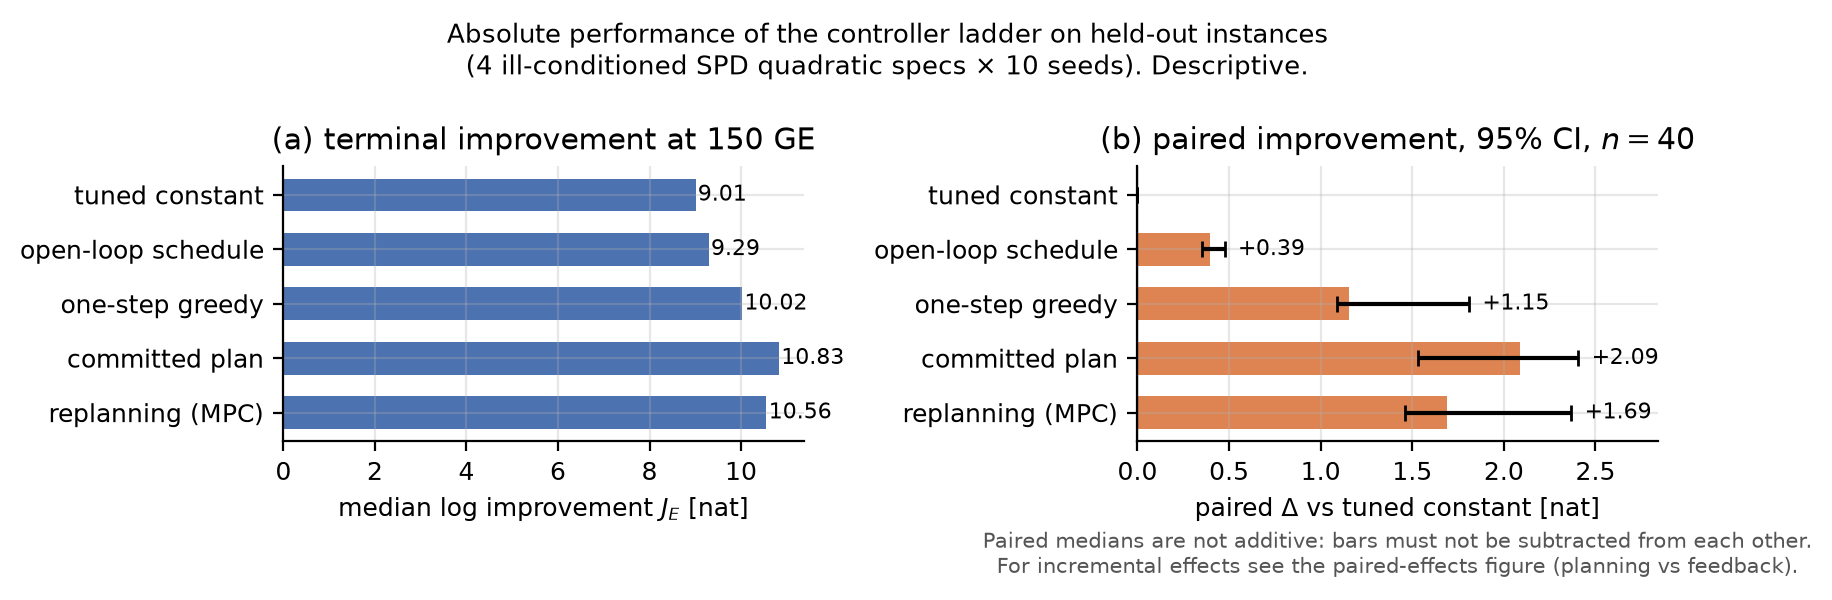
\includegraphics[width=\textwidth]{figure1_ladder.png}
  \caption{Absolute performance across the ladder. This figure describes levels
  only. \textbf{Do not subtract bars in panel (b);} the median of paired
  differences is not linear, so the causal decomposition must be read from
  Figure~\ref{fig:planning-vs-feedback} instead.}
  \label{fig:ladder}
\end{figure}

\subsection{Multi-step lookahead beats one-step}
\label{sec:c2}

$\gate{C2} = +0.456$~nat with a CI lower bound of $+0.254$, above the GO threshold
of $0.3$. Both required conditions were met:

\begin{center}
\begin{tabular}{lr}
\toprule
Condition & Value \\
\midrule
Improvement & $+0.456$~nat, $35/40$ positive \\
Adoption rate of depth $> 1$ & 0.84 \\
Plan-depth cap reached & 0.00 \\
\bottomrule
\end{tabular}
\end{center}

No step failed to consume its quota because of a computational cap, so the
quota-ladder comparison is not compromised.

On development seeds this was conditional ($+0.251$, $p = 0.0771$). At $n = 40$ it
was promoted to GO.

\subsection{Replanning during execution}
\label{sec:c3}

$\gate{C3} = +0.010$~nat, 95\% CI $[-0.033, +0.053]$, with 21 wins, 1 tie, and 18
losses. The CI width of $0.086$~nat is an order of magnitude narrower than the
$0.906$~nat of \gate{A2}.

\begin{quote}
In the held-out results the feedback effect was $+0.010$~nat with a 95\%
confidence interval of $[-0.033, +0.053]$ that narrowly included zero. We
therefore \emph{did not observe a practically large feedback benefit}.
\end{quote}

We do not claim equivalence. Because we did not preregister an equivalence margin,
we cannot report ``the effect is zero'' or ``the effect is smaller than
$0.053$~nat'' as a test result. The two one-sided tests procedure requires bounds
fixed in advance \citep{schuirmann1987tost}, and specifying those bounds ahead of
time is the recommended practice \citep{lakens2017equivalence}.

\subsection{The action space is not the bottleneck}
\label{sec:actionspace}

\ctrl{absolute} (132 actions, $\log_{10}$ range 15.27) gains $+0.005$~nat over
\ctrl{narrow} (12 actions, range 0.95), and $\ctrl{wide} - \ctrl{narrow}$ is
$-0.001$~nat; see Table~\ref{tab:heldout-paired} for intervals. Letting damping be
chosen freely does not raise one-step performance. \emph{This is a negative result,
but it justifies the inexpensive narrow action space.}

The GO threshold for \gate{B} was $0.5$~nat and the observation is two orders of
magnitude smaller, so the verdict is \emph{redesign}. The interval includes zero,
but we make no equivalence claim, for the reason given in Section~\ref{sec:c3}.

\Needspace{6\baselineskip}
\subsection{Search cost}
\label{sec:cost}

\begin{table}[!ht]
  \centering
  % 이 파일은 scripts/make_tables.py 가 생성한다. **손으로 수정하지 않는다.**
% 표: decision-search cost
% raw: headroom_challenge-heldout_step_size_fixed_b8_9a18b6e9.jsonl
% raw 의 SHA-256 은 paper/evidence_map.md 에 있다.
% 공개 저장소에는 raw 가 없다. results/public/*.csv 에서 --public-dir 로 만들면
% 이 파일과 바이트 단위로 같아진다 (scripts/verify_public_results.py).
\begin{tabular}{lrr}
\toprule
Controller & Decision-search GE & Relative to budget \\
\midrule
\texttt{best\_static} & 0 & -- \\
\texttt{best\_open\_loop} & 0 & -- \\
\texttt{heuristic} & 0 & -- \\
\texttt{onestep\_narrow} & 1,186 & $7.9\times$ \\
\texttt{onestep\_absolute} & 10,084 & $67.2\times$ \\
\texttt{committed\_Q4\_narrow} & 69,401 & $462.7\times$ \\
\texttt{shrinking\_Q4\_narrow} & 194,095 & $1,294.0\times$ \\
\bottomrule
\end{tabular}

  \caption{Median decision-search cost on held-out instances, relative to the
  $150$~GE deployment budget. The reported headroom was obtained by an oracle that
  consumed $1{,}294$ times the deployment budget; Section~\ref{sec:cheap} discusses
  what that cost gap implies.}
  \label{tab:heldout-cost}
\end{table}

\section{Where does the headroom come from?}
\label{sec:decomposition}

\textbf{The median of paired differences is not linear.} The values below therefore
do not decompose into a single sum, and each must be read as an
\emph{independently measured statistic}.

\begin{table}[!ht]
  \centering
  % 이 파일은 scripts/make_tables.py 가 생성한다. **손으로 수정하지 않는다.**
% 표: ladder vs tuned constant (직접 측정만)
% raw: headroom_challenge-heldout_step_size_fixed_b8_9a18b6e9.jsonl
% raw 의 SHA-256 은 paper/evidence_map.md 에 있다.
% 공개 저장소에는 raw 가 없다. results/public/*.csv 에서 --public-dir 로 만들면
% 이 파일과 바이트 단위로 같아진다 (scripts/verify_public_results.py).
\begin{tabular}{llrrrr}
\toprule
& Comparison & Median & 95\% CI & $p$ & Positive \\
\midrule
\multicolumn{6}{l}{\emph{Relative to the tuned constant setting}} \\
 & open\_loop & $+0.395$ & $[+0.350, +0.476]$ & ${<}0.0001$ & 40/40 \\
 & onestep\_narrow & $+1.155$ & $[+1.092, +1.811]$ & ${<}0.0001$ & 40/40 \\
 & committed\_Q4\_narrow & $+2.090$ & $[+1.532, +2.407]$ & ${<}0.0001$ & 40/40 \\
 & shrinking\_Q4\_narrow & $+1.690$ & $[+1.462, +2.368]$ & ${<}0.0001$ & 40/40 \\
\midrule
\multicolumn{6}{l}{\emph{Directly measured increments}} \\
C2 & shrinking $-$ onestep & $+0.456$ & $[+0.254, +0.720]$ & ${<}0.0001$ & 35/40 \\
C3 & shrinking $-$ committed & $+0.010$ & $[-0.033, +0.053]$ & $0.9725$ & 21/40 \\
\bottomrule
\end{tabular}

  \caption{Held-out results ($n = 40$). The upper block reports each rung against
  the tuned constant setting; the lower block reports the increments we measured
  \emph{directly}. \textbf{Do not subtract entries across blocks.}}
  \label{tab:ladder}
\end{table}

\begin{figure}[!ht]
  \centering
  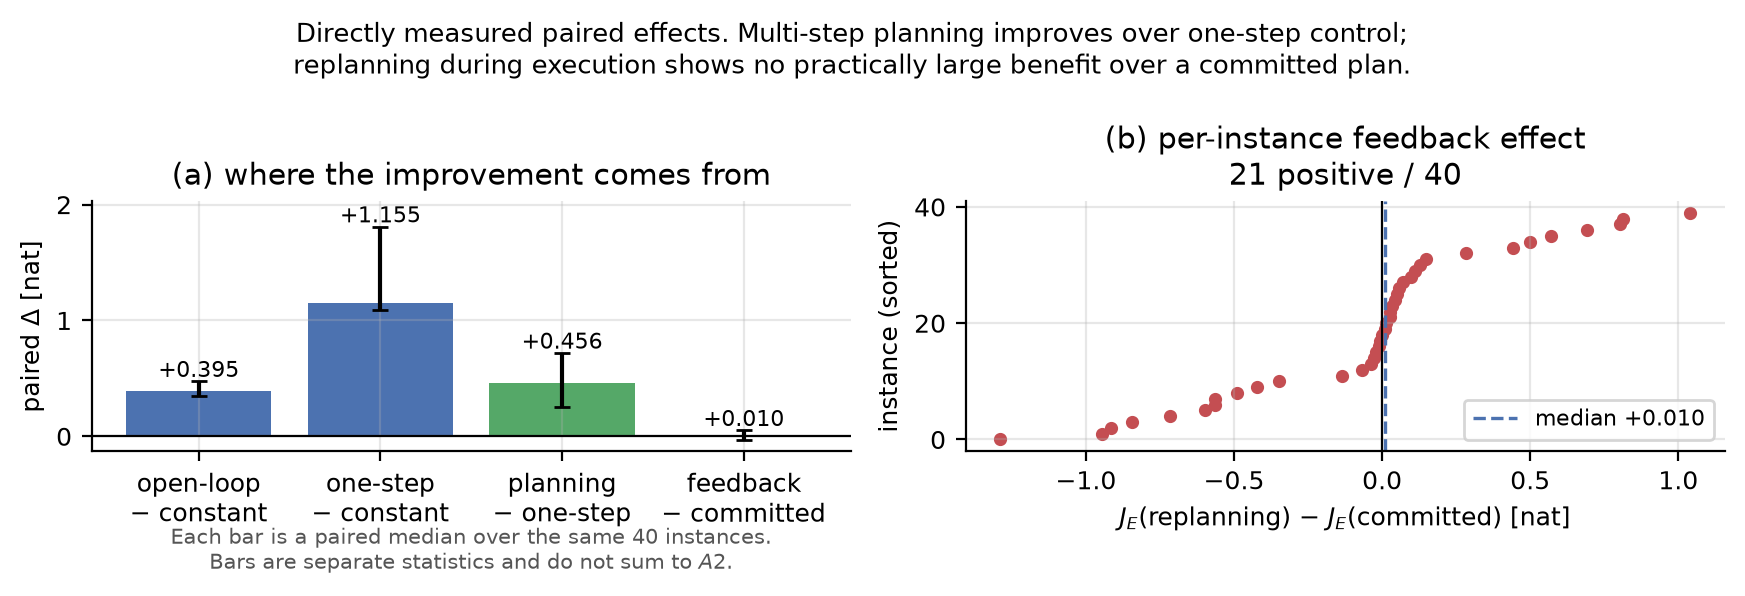
\includegraphics[width=\textwidth]{figure2_planning_vs_feedback.png}
  \caption{Causal decomposition. Only directly measured paired statistics appear
  here. \textbf{Do not subtract bars in panel (a).}}
  \label{fig:planning-vs-feedback}
\end{figure}

\subsection{Why the table entries must not be subtracted}
\label{sec:no-subtraction}

The value of \ctrl{committed} against the constant baseline ($+2.090$) exceeds that
of \ctrl{shrinking} ($+1.690$). Yet the directly measured
$\ctrl{shrinking} - \ctrl{committed}$ is $+0.010$. The two statements are not
contradictory.

\begin{center}
\begin{tabular}{lrrrr}
\toprule
$\ctrl{shrinking} - \ctrl{committed}$ by spec
  & $\kappa{=}10^3$ & $\kappa{=}10^4$ & $\kappa{=}10^5$ & $\kappa{=}10^6$ \\
\midrule
Median & $+0.472$ & $-0.019$ & $+0.009$ & $+0.000$ \\
\bottomrule
\end{tabular}
\end{center}

Within each spec the two planners are effectively tied. The pooled medians fall on
different instances, which is what produces the marginal gap between $+2.090$ and
$+1.690$. \emph{Comparisons are made only with direct paired statistics.} The same
warning appears in Figure~\ref{fig:ladder}.

An earlier version of this manuscript computed the constant-relative value of
\ctrl{onestep} as $\gate{A2} - \gate{C2} = 1.690 - 0.456 = 1.233$. \textbf{That was
wrong.} The directly measured value is $+1.155$.

\subsection{Qualitative conclusion}

\begin{center}
\begin{tabularx}{\linewidth}{@{}Xl@{}}
\toprule
Capability & Directly measured value \\
\midrule
State-dependent control itself (constant $\rightarrow$ one-step)
  & $+1.155$, largest single contribution \\
Increment from multi-step lookahead (one-step $\rightarrow$ planner)
  & $+0.456$, CI lower bound $+0.254$ \\
Increment from replanning (committed $\rightarrow$ planner)
  & $+0.010$, CI $[-0.033, +0.053]$ \\
\bottomrule
\end{tabularx}
\end{center}

\textbf{Q1} is supported. \textbf{Q2} is not supported under these conditions.

\section{Conditioning (exploratory)}
\label{sec:conditioning}

\begin{table}[!ht]
  \centering
  % 이 파일은 scripts/make_tables.py 가 생성한다. **손으로 수정하지 않는다.**
% 표: A2 by condition number
% raw: headroom_challenge-heldout_step_size_fixed_b8_9a18b6e9.jsonl
% raw 의 SHA-256 은 paper/evidence_map.md 에 있다.
% 공개 저장소에는 raw 가 없다. results/public/*.csv 에서 --public-dir 로 만들면
% 이 파일과 바이트 단위로 같아진다 (scripts/verify_public_results.py).
\begin{tabular}{lrrr}
\toprule
Spec & Median & 95\% CI & Positive \\
\midrule
$\kappa = 10^{3}$ & $+6.983$ & $[+6.956, +7.101]$ & 10/10 \\
$\kappa = 10^{4}$ & $+2.317$ & $[+1.529, +2.507]$ & 10/10 \\
$\kappa = 10^{5}$ & $+1.399$ & $[+0.953, +1.517]$ & 10/10 \\
$\kappa = 10^{6}$ & $+1.253$ & $[+0.966, +1.693]$ & 10/10 \\
\bottomrule
\end{tabular}

  \caption{\gate{A2} by spec, $n = 10$ each. Exploratory: the specs were not
  designed as a factorial study of the condition number.}
  \label{tab:conditioning}
\end{table}

\begin{quote}
Adaptive headroom did not increase monotonically with condition number; the largest
effect was observed at $\kappa = 10^3$. This suggests that condition number alone
does not explain the headroom.
\end{quote}

We also do not claim a monotone relation in the opposite direction. The damping
grid, the CG budget, the initial gradient alignment, and the spectral distribution
may all contribute.

\section{Model mismatch (exploratory)}
\label{sec:mismatch}

\subsection{Design}

The results of Section~\ref{sec:heldout} were obtained on deterministic objectives.
Under those conditions the planner's internal model is exact, so the plan formed at
the initial state is already the optimal prediction and replanning cannot acquire
new information. Two readings of $\gate{C3} \approx 0$ are therefore possible:

\begin{description}
  \item[Reading 1] Feedback has no value to begin with.
  \item[Reading 2] This task family is predictable, so feedback was not needed.
\end{description}

The pivotal question is not ``is the model nonlinear?'' but \emph{``is the future
state unpredictable at the time the initial plan is formed?''} We therefore changed
only the samples the optimizer observes, for \emph{the same model and data}:

\begin{center}
\begin{tabular}{ll}
\toprule
Regime & Description \\
\midrule
R1 full-batch & gradients and HVPs over the full dataset; deterministic \\
R2 minibatch  & a fixed-seed batch sequence; the sample changes every step \\
\bottomrule
\end{tabular}
\end{center}

R2 places subsampled curvature inside Newton--CG, a setting known to be difficult
in its own right \citep{byrd2011stochastic}. Our aim is not to resolve that
difficulty but to see whether the value of replanning changes when the planner's
internal predictive model is wrong.

The problem is a two-layer MLP ($4{,}869$ parameters) on a five-class
classification task with $512$ samples generated by a fixed teacher network. The
evaluation objective is always the full dataset, so $\JE$ remains comparable across
regimes.

Batches advance \emph{only after an actual step}. They do not advance during the
planner's look-ahead simulation, so the planner predicts the future using the
current batch. Letting it see future batches would amount to oracle knowledge of
the data and would defeat the purpose of R2.

\Needspace{6\baselineskip}
\subsection{Results}

\begin{table}[!ht]
  \centering
  % 이 파일은 scripts/make_tables.py 가 생성한다. **손으로 수정하지 않는다.**
% 표: micro-neural absolute
% raw: headroom_micro-neural_step_size_fixed_b8_0bec1125.jsonl
% raw 의 SHA-256 은 paper/evidence_map.md 에 있다.
% 공개 저장소에는 raw 가 없다. results/public/*.csv 에서 --public-dir 로 만들면
% 이 파일과 바이트 단위로 같아진다 (scripts/verify_public_results.py).
\begin{tabular}{lrrr}
\toprule
Controller & R1 full-batch & R2 batch 128 & R2 batch 64 \\
\midrule
\texttt{best\_static} & 5.220 & 3.765 & 3.029 \\
\texttt{best\_open\_loop} & 3.299 & 2.100 & 2.984 \\
\texttt{heuristic} & 5.105 & 2.162 & 0.986 \\
\texttt{onestep\_narrow} & 19.886 & 4.296 & 3.468 \\
\texttt{onestep\_absolute} & 19.460 & 4.642 & 3.732 \\
\texttt{committed\_Q4\_narrow} & 20.491 & -0.402 & 1.086 \\
\texttt{shrinking\_Q4\_narrow} & 20.395 & 3.185 & 2.757 \\
\bottomrule
\end{tabular}

  \caption{Absolute median $\JE$ on the micro-neural problem, $n = 3$ per regime.
  Exploratory.}
  \label{tab:micro-absolute}
\end{table}

\begin{table}[!ht]
  \centering
  % 이 파일은 scripts/make_tables.py 가 생성한다. **손으로 수정하지 않는다.**
% 표: micro-neural paired delta (exploratory, n=3 per regime)
% raw: headroom_micro-neural_step_size_fixed_b8_0bec1125.jsonl
% raw 의 SHA-256 은 paper/evidence_map.md 에 있다.
% 공개 저장소에는 raw 가 없다. results/public/*.csv 에서 --public-dir 로 만들면
% 이 파일과 바이트 단위로 같아진다 (scripts/verify_public_results.py).
\begin{tabular}{lrrr}
\toprule
Comparison & R1 full-batch & R2 batch 128 & R2 batch 64 \\
\midrule
shrinking $-$ best\_static & $+15.176$ (3/3) & $-0.900$ (1/3) & $-0.277$ (1/3) \\
shrinking $-$ onestep & $+0.547$ (2/3) & $-1.111$ (1/3) & $-0.716$ (1/3) \\
shrinking $-$ committed & $-0.095$ (1/3) & $+2.941$ (3/3) & $+1.666$ (3/3) \\
committed $-$ onestep & $+0.470$ (2/3) & $-4.444$ (0/3) & $-2.322$ (0/3) \\
\bottomrule
\end{tabular}

  \caption{Paired differences by regime. \emph{We do not quote confidence
  intervals or $p$-values} at $n = 3$; the parenthesized figure is the count of
  positive pairs.}
  \label{tab:micro-paired}
\end{table}

\subsection{Why $\gate{C3} > 0$ in R2}
\label{sec:c3-r2}

The absolute values distinguish the two readings:

\begin{center}
\begin{tabular}{lrrr}
\toprule
Controller & R1 & R2 (batch 64) & R2 (batch 128) \\
\midrule
\ctrl{committed} & 20.491 & 1.086 & $-0.402$ \\
\ctrl{shrinking} & 20.395 & 2.757 & 3.185 \\
\bottomrule
\end{tabular}
\end{center}

In R2, \ctrl{committed} falls below even \ctrl{best\_static} and trails
\ctrl{onestep} by $2.3$ to $4.4$~nat. The rejection rate is decisive.

\begin{figure}[!ht]
  \centering
  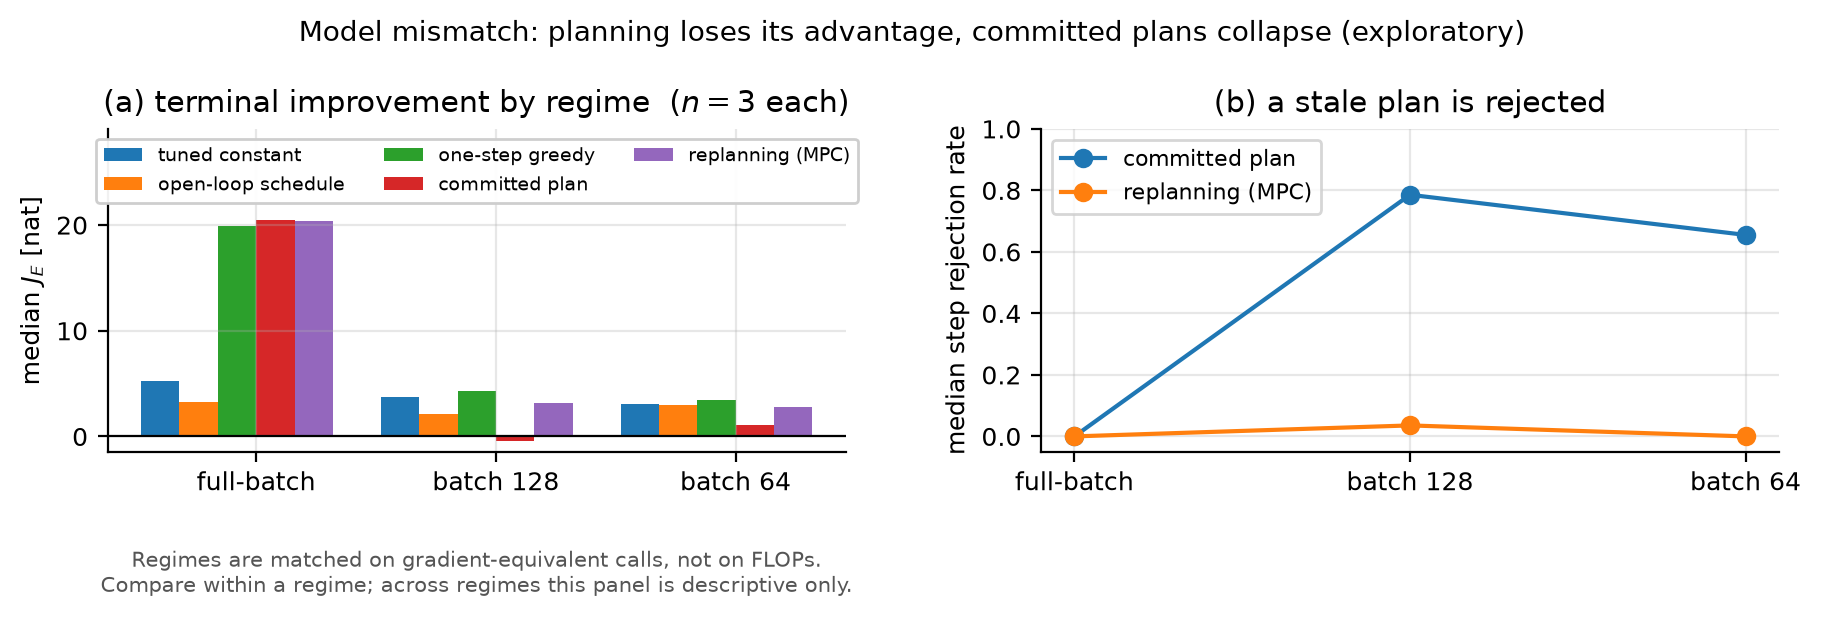
\includegraphics[width=\textwidth]{figure3_model_mismatch.png}
  \caption{Exploratory micro-neural results under model mismatch, $n = 3$ per
  regime. Panel (a) compares terminal improvement across the full-batch and
  minibatch regimes. Panel (b) gives the rejection rate of \ctrl{committed}:
  $0.00$ in R1, $0.79$ at batch 128, $0.66$ at batch 64, so a large fraction of
  the plan formed at the initial state is rejected by later batches.}
  \label{fig:mismatch}
\end{figure}

That is, $\gate{C3} > 0$ does not mean \ctrl{shrinking} became better; it means
\emph{holding a stale plan is costly}.

At the same time, in R2 the planner falls below both the tuned constant and the
inexpensive one-step controller. State-conditioned control does help in R2
(\ctrl{onestep} $3.468$ versus \ctrl{best\_static} $3.029$), but one-step greedy
control already provides it at $1/146$ of the planner's search cost (batch-64
regime medians: \ctrl{onestep} $1{,}879$~GE, \ctrl{shrinking} $275{,}286$~GE).

\subsection{Limitations of this experiment}

\begin{itemize}
  \item $n = 3$ per regime. We do not quote CIs or $p$-values.
  \item The transition across three batch sizes is not monotone: batch 128 scores
        below batch 64.
  \item Cross-regime absolute comparisons are not FLOP-normalized
        (Section~\ref{sec:ge}).
  \item One model, one dataset.
\end{itemize}

The R1 value $\gate{C2} = +0.547$ agrees in sign with the $+0.456$ of
Section~\ref{sec:heldout} ($n = 40$, $p < 0.0001$), but becomes $-0.080$ under the
alternative acceptance criterion. The $n = 40$ result is the stronger one and
$n = 3$ does not overturn it. \emph{We report the disagreement itself as a result.}

\section{Acceptance criterion ablation (exploratory)}
\label{sec:ablation}

\subsection{Motivation}

The R2 results of Section~\ref{sec:mismatch} mix two effects:

\begin{enumerate}
  \item the initial plan going stale as the minibatch changes;
  \item steps being rejected because monotone decrease is required on a noisy
        objective.
\end{enumerate}

The default acceptance rule requires monotone decrease of the current minibatch
objective. A step that improves the true objective can be rejected because of
sample noise.

\subsection{Design}

\begin{quote}
We replaced minibatch-local monotonic acceptance with a fixed-evaluation-objective
criterion.
\end{quote}

Gradients and HVPs are still computed on the minibatch. Only the acceptance test
changes. A forward pass on the fixed evaluation objective costs
$n_{\text{samples}} / \text{batch size}$ times more, and that factor is included in
the GE accounting.

\subsection{Results}

\begin{table}[!ht]
  \centering
  % 이 파일은 scripts/make_tables.py 가 생성한다. **손으로 수정하지 않는다.**
% 표: acceptance criterion ablation (exploratory, n=3 per regime)
% raw: headroom_micro-neural_step_size_fixed_b8_0bec1125.jsonl
% raw: headroom_micro-neural_step_size_fixed_b8_9f3194be.jsonl
% raw 의 SHA-256 은 paper/evidence_map.md 에 있다.
% 공개 저장소에는 raw 가 없다. results/public/*.csv 에서 --public-dir 로 만들면
% **고정된 환경에서** 이 파일과 바이트 단위로 같아진다.
% 판본이 다른 환경에서의 비트 수준 일치는 주장하지 않는다.
\begin{tabular}{lllrr}
\toprule
Gate & Regime & & Control & Fixed evaluation \\
\midrule
A2 & R1 full-batch & & $+15.176$ (3/3) & $+14.065$ (3/3) \\
 & R2 batch 128 & & $-0.900$ (1/3) & $-0.598$ (0/3) \\
 & R2 batch 64 & & $-0.277$ (1/3) & $-0.093$ (0/3) \\
\midrule
C2 & R1 full-batch & & $+0.547$ (2/3) & $-0.080$ (1/3) \\
 & R2 batch 128 & & $-1.111$ (1/3) & $-0.118$ (1/3) \\
 & R2 batch 64 & & $-0.716$ (1/3) & $+0.104$ (2/3) \\
\midrule
C3 & R1 full-batch & & $-0.095$ (1/3) & $-0.949$ (0/3) \\
 & R2 batch 128 & & $+2.941$ (3/3) & $+1.110$ (3/3) \\
 & R2 batch 64 & & $+1.666$ (3/3) & $+0.973$ (3/3) \\
\bottomrule
\end{tabular}

  \caption{Paired differences under the two acceptance criteria, $n = 3$ per
  regime. Exploratory.}
  \label{tab:acceptance-delta}
\end{table}

\begin{figure}[!ht]
  \centering
  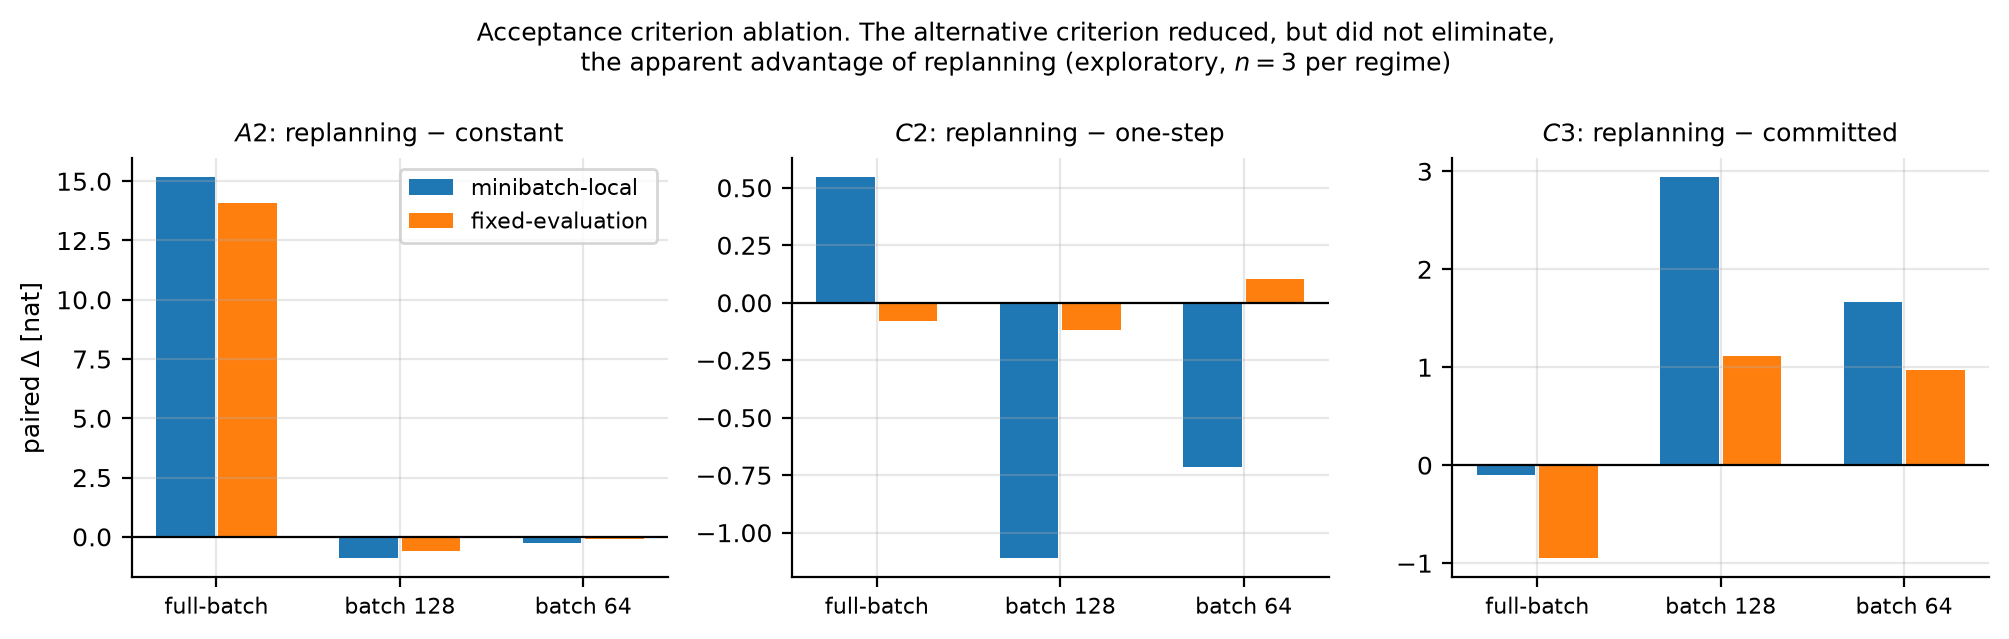
\includegraphics[width=\textwidth]{figure4_acceptance_ablation.png}
  \caption{Paired \gate{A2}, \gate{C2} and \gate{C3} effects under minibatch-local
  and fixed-evaluation acceptance, $n = 3$ per regime. The alternative criterion
  reduced, but did not eliminate, the apparent advantage of replanning over a
  committed stale plan, and \ctrl{shrinking} did not establish an advantage over
  \ctrl{onestep}. Exploratory.}
  \label{fig:acceptance}
\end{figure}

\begin{quote}
This alternative criterion reduced, but did not eliminate, the apparent advantage
of replanning over a committed stale plan. The estimated $\gate{C3}$ magnitude
decreased substantially under the alternative acceptance criterion, indicating that
the original magnitude was partly acceptance-dependent.
\end{quote}

In R2, \ctrl{shrinking} still does not beat \ctrl{best\_static} (zero of three
pairs positive) and only draws level with \ctrl{onestep}.

\subsection{The alternative criterion was stricter, not looser}
\label{sec:stricter}

\begin{table}[!ht]
  \centering
  % 이 파일은 scripts/make_tables.py 가 생성한다. **손으로 수정하지 않는다.**
% 표: rejection rate under two acceptance criteria
% raw: headroom_micro-neural_step_size_fixed_b8_0bec1125.jsonl
% raw: headroom_micro-neural_step_size_fixed_b8_9f3194be.jsonl
% raw 의 SHA-256 은 paper/evidence_map.md 에 있다.
% 공개 저장소에는 raw 가 없다. results/public/*.csv 에서 --public-dir 로 만들면
% 이 파일과 바이트 단위로 같아진다 (scripts/verify_public_results.py).
\begin{tabular}{llrr}
\toprule
Controller & Regime & Control & Fixed evaluation \\
\midrule
\texttt{committed} & R1 full-batch & 0.00 & 0.04 \\
 & R2 batch 128 & 0.79 & 0.89 \\
 & R2 batch 64 & 0.66 & 0.92 \\
\midrule
\texttt{shrinking} & R1 full-batch & 0.00 & 0.04 \\
 & R2 batch 128 & 0.04 & 0.42 \\
 & R2 batch 64 & 0.00 & 0.36 \\
\midrule
\texttt{onestep} & R1 full-batch & 0.04 & 0.04 \\
 & R2 batch 128 & 0.03 & 0.53 \\
 & R2 batch 64 & 0.00 & 0.57 \\
\bottomrule
\end{tabular}

  \caption{Median rejection rate under the two acceptance criteria. Rejection rates
  \emph{rose} under the alternative criterion.}
  \label{tab:acceptance-rejection}
\end{table}

Under the default rule, \texttt{loss\_before} and the candidate losses live on
\emph{the same minibatch}. Reducing the loss of the batch whose gradient was just
computed is easy. The alternative criterion requires a decrease in the full-data
loss and therefore blocks steps that overfit the current batch.

\subsection{Limitations of this ablation}
\label{sec:ablation-limits}

\textbf{This is not a single-factor change.} The acceptance criterion and the
number of effective steps change together. Excluding the evaluation cost from the
accounting would hide a real cost, so we included it, and the price is that the two
effects are entangled. We therefore \emph{do not use absolute comparisons between
the two columns to argue that one acceptance rule is better}.

The R1 column is not a meaningful comparison. In the full-batch regime the fixed
evaluation objective and the curvature objective take the same value, so all the
alternative criterion changes is charging one extra forward pass per step
(\ctrl{best\_static}: $5.2199 \rightarrow 5.1094$). That is a budget perturbation.

\section{Why we did not train a policy}
\label{sec:nopolicy}

This section separates two things: the scientific conclusion the data supports, and
a project decision about resource commitment.

\subsection{Scientific conclusion}
\label{sec:scientific-conclusion}

\begin{enumerate}
  \item Multi-step planning improved over one-step control on held-out instances
        ($+0.456$~nat, CI $+0.254$ to $+0.720$, $35/40$).
  \item Replanning during execution did not meaningfully improve over committed
        planning: $+0.010$~nat, $21/40$.

        \begin{quote}
        The confidence interval was narrow and included zero, and we did not
        observe a practically large feedback benefit.
        \end{quote}

        We do not write ``equivalent'' or ``statistically the same''; there is no
        prior equivalence margin
        \citep{schuirmann1987tost,lakens2017equivalence}.
  \item Under stochastic model mismatch the committed plan was fragile. The
        rejection rate rose from $0.00$ to $0.66$--$0.79$ and terminal improvement
        fell below the tuned constant.
  \item Replanning reduced that fragility but did not consistently outperform
        inexpensive one-step control: $\text{replanning} - \text{one-step}$ was
        $-1.111$ and $-0.716$ in the two minibatch conditions
        ($n = 3$ per regime, exploratory).
\end{enumerate}

\subsection{Project decision}

\begin{quote}
PPO training was a conditional next stage, not a required component of the study. We
predeclared empirical gates to determine whether the added implementation and
computational cost was justified. Because feedback replanning did not consistently
outperform committed planning or inexpensive one-step control, we did not proceed to
PPO.
\end{quote}

That decision-search cost is $1{,}294$ times the deployment budget also enters this
judgement.

We state the distinction explicitly:

\begin{itemize}
  \item PPO did not fail.
  \item We did not run PPO.
  \item This is not a rejection of reinforcement learning in general.
  \item We did not establish headroom that would justify a learned state-dependent
        feedback policy in the present environment.
\end{itemize}

\subsection{The status of the gates}

The gate thresholds (for example $\gate{C3} \geq 0.3$~nat) are \emph{not} universal
theoretical criteria. Their character is as follows:

\begin{itemize}
  \item Policy learning requires a separate, large experimental stage.
  \item We therefore registered in advance a minimum effect size, a sign-consistency
        requirement, whether multi-step plans were used, and transfer conditions.
  \item The gates are a scope-control device, not a statistical truth verdict.
  \item We did not change the thresholds after seeing results.
\end{itemize}

The thresholds were fixed before the results were seen and were not changed
afterwards. Their particular values are a scope-control choice, not a claim of
correctness.

\subsection{Follow-up direction}
\label{sec:followup}

That \gate{C2} is GO on held-out instances means a good multi-step sequence exists,
and that \gate{C3} is small means that sequence can be determined at the initial
state. This combination points less towards a per-step feedback policy than towards
an \emph{amortized approach that predicts a schedule from initial problem features}
\citep{amos2023amortized,andrychowicz2016l2l,bae2022apo}. We did not implement it
and mention it only as a direction.

\section{Discussion}
\label{sec:discussion}

\subsection{Planning is not feedback}
\label{sec:planning-not-feedback}

Each rung of the ladder measures the value of a different capability:

\begin{center}
\begin{tabular}{ll}
\toprule
Rung & Capability measured \\
\midrule
constant $\rightarrow$ one-step   & value of immediate per-state selection \\
one-step $\rightarrow$ committed  & value of multi-step lookahead \\
committed $\rightarrow$ replanning & value of revising the plan during execution \\
\bottomrule
\end{tabular}
\end{center}

\textbf{We do not decompose these values arithmetically.} The median of paired
differences is not linear. In our measurements \ctrl{committed} is $+2.090$ and
replanning is $+1.690$ against the tuned constant, yet the directly measured
$\text{replanning} - \ctrl{committed}$ is $+0.010$. By spec the values are
$+0.472 / -0.019 / +0.009 / +0.000$, so the two planners are effectively tied and
the marginal gap arises because the pooled medians fall on different instances.
\emph{Comparisons are made only with direct paired statistics}
(Section~\ref{sec:no-subtraction}, Figure~\ref{fig:planning-vs-feedback}).

\textbf{Q1} (does a good sequence exist?) is supported; \textbf{Q2} (is it worth
revising during execution?) is not supported under these conditions. On a
deterministic objective the planner's internal model is exact, so the plan formed at
the initial state is already the optimal prediction and replanning gains no new
information.

\subsection{Model error raises the risk of long-horizon plans}
\label{sec:model-error}

The exploratory micro-neural results summarize as follows.

\begin{quote}
Long-horizon plans are valuable when the internal predictive model is accurate; when
the model is wrong, the risk of a stale plan grows.
\end{quote}

In the minibatch regimes the rejection rate of the committed plan rose from $0.00$ to
$0.66$--$0.79$ and terminal improvement fell below the tuned constant. Replanning
reduced that loss.

\textbf{Yet under the same conditions replanning is worse than one-step control.}
$\text{replanning} - \text{one-step}$ is $-1.111$ and $-0.716$ in the two minibatch
conditions, and $\text{replanning} - \text{tuned constant}$ is $-0.900$ and $-0.277$.
So one must not read the positive $\ctrl{committed} \rightarrow \text{replanning}$
value as evidence for a learned feedback policy. \emph{That positive value is
stale-plan avoidance, not an advantage over inexpensive myopic control.}

At $n = 3$ per regime we make no claim about magnitude.

\subsection{Why the benchmark audit was necessary}
\label{sec:audit-why}

\begin{quote}
Our benchmark audit was necessary because nominal numerical ceilings and task labels
did not reliably identify whether a problem could distinguish controllers.
\end{quote}

These are the problems that actually reversed conclusions in this project:

\begin{itemize}
  \item joint saturation at the numerical floor (two of three specs in the initial
        dev subset);
  \item one-sided saturation, where dropping pairs removed the good results;
  \item an attainable local minimum of Rosenbrock, which passed the eligibility
        check;
  \item identical seeds producing identical instances, so a nominal $n = 3$ was
        $n = 1$;
  \item the difference between a ceiling based on the global optimum and one based on
        the starting-point basin;
  \item the possibility that a single reference solver fails (L-BFGS did not
        converge at $\kappa = 10^6$).
\end{itemize}

Both of our initial rules --- ``judge saturation from the task name'' and ``compute
the ceiling from the numerical floor'' --- were wrong. That is why we introduced the
reference-solver panel and the attainable ceiling.

\textbf{We are not proposing a general benchmark framework.} This is an empirical
procedure that corrected this project's benchmark, and we intend it to be read as a
checklist to consult when designing similar controller comparisons.

\subsection{What the cheap method misses}
\label{sec:cheap}

\ctrl{onestep} spends $7.9$ times the budget on search --- $1/164$ of the planner
--- and gains $+1.155$~nat over the tuned constant. The planner gains $+1.690$~nat
but spends $1{,}294$ times the budget. The directly measured increment of
$+0.456$~nat is statistically robust, but this cost gap is its price. From a
practical standpoint this is the most direct implication of the present results.

\section{Limitations}
\label{sec:limitations}

\subsection{What we do not claim}

\begin{center}
\begin{tabular}{p{0.42\textwidth}p{0.52\textwidth}}
\toprule
Claim we avoid & Why \\
\midrule
``feedback is useless'' / ``we established a zero effect''
  & No equivalence margin was preregistered. We use only the wording of
    Section~\ref{sec:c3}. \\
``exactly half of \gate{C3} was an acceptance artifact''
  & The reduction differs by regime (62\%, 42\%) and $n = 3$. We use only the wording
    of Section~\ref{sec:ablation}. \\
``reinforcement learning fails at optimizer control''
  & We did not train a policy. \\
``the deterministic setting is $N$ times better than the stochastic one''
  & GE does not match FLOPs across batch sizes (Section~\ref{sec:ge}). \\
``headroom decreases with condition number''
  & We observed non-monotonicity only. We claim monotonicity in neither direction. \\
``the method fails on nonlinear problems''
  & Both Rosenbrock variants were ruled unusable as benchmark defects. \\
``the micro-neural results overturn the quadratic results''
  & $n = 3$ exploratory versus $n = 40$ held-out. \\
Any value formed by adding or subtracting paired medians
  & The median is not linear. Comparisons use direct paired measurements only
    (Section~\ref{sec:no-subtraction}). \\
\bottomrule
\end{tabular}
\end{center}

\subsection{Protocol deviations}
\label{sec:deviations}

\begin{description}
  \item[E1] The configuration selection rule was finalized after inspecting the gate
    table of a single-instance dry run (Section~\ref{sec:deviation-selection}).
  \item[E2] (quad $\kappa{=}10^5$, seed 2) overlaps between the initial dev audit and
    configuration selection (Section~\ref{sec:seeds}).
  \item[E3] Some executions ran with uncommitted changes, recorded as
    \texttt{code\_dirty}.
  \item[E4] Tests ran concurrently with the held-out execution. Wall-clock records are
    therefore inaccurate, but numerical results and verdicts are unaffected
    (single-threaded deterministic arithmetic).
  \item[E5] Summary-level provenance omitted the commit field because of a reporting
    bug; the corresponding per-run raw records retained the commit, allowing
    deterministic reconstruction.
  \item[E6] The acceptance-criterion ablation is not a single-factor change
    (Section~\ref{sec:ablation-limits}).
  \item[E7] The R1 column of the alternative criterion is a budget perturbation
    (Section~\ref{sec:ablation-limits}).
  \item[E8] Gate \gate{C1} uses a single-seed diagnostic baseline and was not used for
    any verdict.
  \item[E9] Three-layer reporting is not applied to gates \gate{A1} and \gate{B},
    which use a single statistic.
  \item[E10] An earlier diagnostic script used an upper-middle convention for even
    sample counts, whereas the main paired analysis used the conventional arithmetic
    median. All reporting code was unified before manuscript generation; the selected
    configuration and qualitative conclusions were unchanged.
  \item[E11] Run identifiers initially embedded the full target table rather than only
    the targets used by the corresponding task family. Adding a target entry for an
    unrelated task family therefore invalidated the cost-to-target runs of the
    quadratic suite. We restricted the identifier to the targets actually used and
    re-executed those runs; the fixed-budget comparisons were unaffected, and the
    cost-to-target statistic is a re-aggregation of the same measurements.
  \item[E12] The protocol specified that a tag be created at the
    configuration-freeze point. The tag exists in the private repository, but it was
    created after the confirmatory runs had completed and it points at the final
    Stage~2 commit rather than at the freeze commit. It therefore cannot attest that
    the configuration was fixed before the held-out runs; that ordering is attested by
    the dated decision record and by the freeze commit itself. We did not move the tag
    retroactively. The tag is not part of the public export: the commit it marks
    precedes the removal of device names from committed artifacts, and the public
    repository does not share history with the private one. It is, however, present on
    the private repository's remote, so withholding it from the export limits the
    exposure to that repository rather than eliminating it.
\end{description}

\subsection{Scope and confounds}
\label{sec:scope}

\begin{description}
  \item[L1] The primary confirmatory results are limited to synthetic ill-conditioned
    SPD quadratics: $d = 100$ fixed, four values of $\kappa$, ten held-out seeds.
  \item[L2] The micro-neural results are exploratory evidence at $n = 3$ per regime.
    We do not quote CIs or $p$-values.
  \item[L3] The acceptance ablation includes the evaluation forward cost and is
    therefore not a single-factor change; the acceptance criterion and the number of
    effective steps change together.
  \item[L4] GE matches oracle calls within a regime, not FLOPs across batch sizes.
    Cross-regime absolute comparisons are descriptive.
  \item[L5] The fixed-evaluation criterion is not a relaxation. Measured rejection
    rates rose under it; it is the stricter rule.
  \item[L6] Beam-search cost is far larger than the object-level budget:
    $194{,}095 \GE / 150 \GE = 1{,}294\times$.
  \item[L7] The selection rule was fixed before the full execution but after
    inspecting the gate table of a cost-measurement dry run. Recorded as a protocol
    deviation (E1).
  \item[L8] We did not run PPO, so we can draw no conclusion about learned-policy
    performance.
  \item[L9] The results do not generalize to Hessian-free Newton methods as a family,
    nor to neural optimization in general.
\end{description}

The Rosenbrock benchmark defect and the median-convention correction appear in
Section~\ref{sec:reproducibility} and in the deviation list above and are not
repeated here.

\section{Reproducibility}
\label{sec:reproducibility}

\subsection{Execution environment}

\begin{quote}
All Stage~2 optimization and planning experiments were executed on CPU. The
GPU-derived cost-model files in the repository originate from an earlier Stage~1
calibration and were not used in Stage~2; Stage~2 GE accounting used HVP-equivalent
oracle counts.
\end{quote}

\begin{quote}
Search GE measures simulated oracle work rather than wall-clock GPU compute.
\end{quote}

Execution was pinned to a single thread. Wall-clock time is used in no verdict.

\subsection{Artifacts}

\begin{center}
\begin{tabular}{ll}
\toprule
Artifact & Location \\
\midrule
Reproduction commands       & \texttt{docs/reproduce.md} \\
Generated result tables     & \texttt{docs/results\_stage2.md} \\
Raw checksums (SHA-256)     & \texttt{paper/evidence\_map.md} \\
Claim ledger                & \texttt{paper/claim\_ledger.md} \\
Citation content checklist  & \texttt{paper/CITATIONS.md} \\
Protocol (decisions D1--D32) & \texttt{docs/experiment\_protocol.md} \\
Tests                       & 497 \\
\bottomrule
\end{tabular}
\end{center}

Of the 497 tests, 465 cover the implementation and 32 cover the published reproduction
package itself: that the row-level result files reproduce the headline numbers above, and
that the accompanying notebook stays runnable.

The code and reproducibility package are published at
\url{https://github.com/bu11ymaguire/When_Does_Feedback_Help}, release tag
\texttt{arxiv-submission-v1}.

That repository is an allowlist export of the verified private source tree; it does not
share Git history with it. The manifest shipped with the export records the private
source commit and a SHA-256 for every exported file, so the two trees can be checked
against each other in one direction without publishing the private history.

The export includes row-level result files sufficient to recompute every paired
statistic reported here. Under the pinned software environment the paired analysis is
deterministic --- it draws $10{,}000$ bootstrap resamples at a fixed seed, using the
Python standard library rather than the numerical stack --- so the reported medians,
confidence intervals, and $p$-values can be recomputed from the public row-level
results. We do not claim bit-level agreement across different library versions or
platforms.

All numbers in this manuscript originate in \texttt{docs/results\_stage2.md}, whose
sources are pinned by the SHA-256 values in \texttt{paper/evidence\_map.md}. The
tables in \texttt{paper/tables/} are generated by
\texttt{scripts/make\_tables.py} from the same raw records and the same median
convention. \textbf{Numbers are not edited by hand in this manuscript.}

The result store skips completed runs. Because identity is separated into three
layers, editing aggregation code or documentation does not cause the optimizer to
rerun.

\subsection*{Privacy note}

\begin{quote}
Hostnames in committed public artifacts were replaced with stable pseudonymous labels
before public release. This sanitization did not modify experimental configurations,
results, checksums of raw numerical records, or scientific conclusions.
\end{quote}

Two repositories must be distinguished here.

\begin{quote}
Earlier hostnames remain in the private source repository's history. The public
reproducibility repository is an allowlist export with independent Git history and
contains only pseudonymous host identifiers.
\end{quote}

The export tool refuses to run if a device name appears in any file it would publish, so
the second sentence is checked mechanically rather than asserted.

\subsection*{AI-Assisted Research Disclosure}

Claude Opus, accessed through Kiro, assisted with implementation, refactoring, test
generation, experiment orchestration, and report generation. GPT-5.6 Sol, accessed
through ChatGPT, assisted with methodological critique, confound analysis, claim
calibration, and manuscript review. The human author formulated the research
questions, approved protocol changes, verified the reported results, determined
their interpretation, and assumes full responsibility for the work.


\bibliographystyle{plainnat}
\bibliography{references}

\end{document}
